\documentclass[fleqn,10pt]{olplainarticle}
% Use option lineno for line numbers 
\setlength{\parindent}{0pt}
\setlength{\parskip}{6pt}
\usepackage{xcolor}
\colorlet{color2}{white}  % olplainarticle 使用 color2 作为 abstract 文字颜色
\bibliographystyle{apalike}
\bibliographystyle{unsrtnat}   % <- orders entries by citation order
\usepackage[colorlinks=true,linkcolor=blue,citecolor=blue,urlcolor=blue]{hyperref}
\usepackage{subcaption}


\title{CSE 6010 CheckPoint 1: \\Campus Navigation System}

\author[1]{Jing He}
\author[2]{Fred Yang}
\author[3]{Haowen Jiang}
\author[4]{Ming-Cheng Fan}
\author[5]{Chia-Hsin Chiu}
\affil[1]{jhe468@gatech.edu}
\affil[2]{fred.yang@gatech.edu}
\affil[3]{hjiang401@gatech.edu}
\affil[4]{mfan77@gatech.edu}
\affil[5]{cchiu73@gatech.edu}

\begin{abstract}
This project presents the development of a vehicle navigation prototype for the Georgia Tech campus, leveraging OpenStreetMap (OSM) as the data source. The campus road network is constructed as a weighted and directed graph, where edge weights represent travel costs such as distance and estimated time. To compute the shortest paths, we use A* Search algorithm as our core algorithm. The prototype is designed to generate two main outputs for users: (1) Estimated travel time, calculated based on segment distances and an assumed vehicle speed, and (2) Turn-by-turn route instructions, which include straight segments, left/right turns, and cumulative distance for each instruction. By combining more useful extensions, we hope to create a fully functional navigation system. 
\end{abstract}

\usepackage[numbers,sort&compress]{natbib}
\makeatletter
\makeatother
\begin{document}

\flushbottom
\maketitle
\thispagestyle{empty}


\section*{Introduction}
Navigation systems are essential for guiding users efficiently to their destinations, improving travel time, safety, and overall convenience. In addition, navigation systems offer users reassurance when traveling in unfamiliar areas, reducing anxiety and enhancing confidence in reaching their destinations. This project is inspired by such systems and aims to develop a vehicle navigation prototype specifically for Georgia Tech campus. By modeling the campus road network as a graph, the system can compute optimal (shortest) routes and provide results including estimated travel time and turn-by-turn instructions. This prototype not only facilitates navigation within a constrained environment but also serves as a foundation for all potential extensions. 

\section*{Literature Review}
Navigation systems play a vital role in improving mobility by enabling users to efficiently reach destinations while reducing travel time and uncertainty. For constrained environments such as university campuses, OpenStreetMap (OSM) has proven to be a reliable open-source dataset for routing applications, as it provides accessible road and building data that can be transformed into graph structures suitable for shortest-path algorithms \cite{10.1007/978-3-642-10601-9_13, s18020509}. Several campus navigation prototypes have successfully applied OSM, highlighting its adaptability for small-scale routing tasks.

Graph-based modeling forms the foundation of most navigation systems, where intersections and road segments are represented as nodes and edges. To connect buildings to the network, geometric techniques such as centroid projection are commonly employed. These approaches are widely used in map-matching research to systematically link arbitrary points, such as building entrances, to accessible roads \cite{Map-mappingResearch}. Once modeled, shortest-path algorithms such as Dijkstra’s and A* are effective for campus-scale applications. While Dijkstra guarantees optimality, A* enhances efficiency by incorporating heuristics like Euclidean distance \cite{madkour2017survey}. Advanced algorithms designed for large-scale, real-time routing (e.g., Contraction Hierarchies) offer limited additional benefit at the campus scale.

Equally important is the generation of user-friendly navigation instructions. Research shows that effective guidance depends on identifying decision points, computing turning angles, and translating them into intuitive directions such as “turn left” or “go straight” \cite{RICHTER2008233}. Studies further emphasize the value of simplicity and landmarks in reducing user disorientation, underlining that navigation is not only a technical problem but also a human-centered design challenge.

In summary, existing literature confirms the feasibility of developing a campus-scale navigation system using OSM data, graph modeling, and classical shortest-path algorithms. Simplified assumptions, such as constant travel speed and geometric building linkage, align with prior work, while future opportunities include integrating landmarks or augmented reality features to improve usability.

\section*{Objectives}
The objective of this project is to create a Georgia Tech campus navigation system, which aims to assist users in finding the shortest route between a starting point and destination. By using a graph-based representation of part of the campus road network, the system provides the shortest path and corresponding instructions. The goal is to demonstrate a vehicle routing prototype that can serve as a foundation for future extension of a full-scale navigation system.

\subsection*{Input}
\begin{itemize}
    \item \textbf{Starting point (From):} The initial location of the vehicle or user, represented as a coordinate pair (latitude, longitude)
    \item \textbf{Destination (To):} The target location to reach, represented as a coordinate pair (latitude, longitude)
\end{itemize}

\subsection*{Output}
\begin{itemize}
    \item \textbf{Estimated travel time}: Calculated based on segment distances and assumed vehicle speed (Total Distance / Vehicle Speed)
    \item \textbf{Shortest-Path Distance}: The shortest-path distance from the starting point to the destination
    \item \textbf{Turn-by-turn route instructions}: Guidance including straight segments, left/right turns, and cumulative distance for each instruction
    \item \textbf{Node and edge sequence}: The ordered list of nodes and edges representing the planned route
    \item \textbf{Bearing angles}: Represent how the actual path is constructed by edges, which are then used to generate instructions
\end{itemize}

\subsection*{Displayed Output}
\begin{itemize}
    \item \textbf{Estimated travel time}: Calculated based on segment distances and assumed vehicle speed (Total Distance / Vehicle Speed)
    \item \textbf{Turn-by-turn route instructions}: Guidance including straight segments, left/right turns, and cumulative distance for each instruction
\end{itemize}

\section*{System Descriptions}
\subsection*{System Scope}
\begin{itemize}
    \item Area: Georgia Tech Atlanta campus
    \item Road network modeled as a graph with nodes representing intersections or key points and edges representing road segments
\end{itemize}

\subsection*{Specific Goals}
\begin{itemize}
    \item Accurately model the campus road network as a graph suitable for shortest-path algorithms
    \item Implement a shortest-path algorithm to generate optimal vehicle routes
    \item Compute total distance and estimated travel time for each route
    \item Generate turn-by-turn route instructions based on the geometry of the road segments (edges)
    \item Provide a clear output that can be used for vehicle navigation or further extension to real-time navigation systems
\end{itemize}

\section*{Data Descriptions}
\subsection*{Data Source}
We aim to construct an adjacency list that captures the connectivity between campus buildings and the surrounding road network, serving as the dataset for our research. The data are obtained from \textbf{OpenStreetMap (OSM)}, an open geospatial platform collaboratively maintained and continuously updated by contributors worldwide. OSM organizes geographic information in a structured format consisting of \textbf{nodes}, \textbf{ways}, and \textbf{relations}:
\begin{itemize}
    \item \textbf{Buildings} are represented as closed polygons, defined by a series of latitude–longitude coordinates (nodes). Each building polygon is associated with descriptive tags, such as \texttt{building=yes} and \texttt{name=Tech Tower}.

    \item \textbf{Roads} are represented as polylines (collections of line segments) defined by ordered nodes. Road attributes include type (e.g., \texttt{highway=primary}, \texttt{highway=residential}) and access restrictions (e.g., \texttt{network\_type=drive}).
\end{itemize}


For this phase, we extracted \textbf{motor-vehicle-accessible roads} (\texttt{network\_type=drive}) within the Georgia Tech campus.

\subsection*{Data Preparation Assumptions}
To connect buildings with the road network, we make the following assumptions:
\begin{enumerate}
    \item \textbf{Parking locations must lie on motor-vehicle roads,} i.e., cars must park alongside the road rather than on arbitrary open areas.
    \item \textbf{Walking distance simplification}: the walking distance is approximated as the straight-line distance between the building centroid and a point on the nearest road segment, instead of using the actual pedestrian path network.
    \item \textbf{Definition of shortest distance}: for each road, the shortest distance from the building centroid is defined as the \textbf{point-to-line-segment projection distance}, rather than simply the Euclidean distance to an endpoint of the road.
\end{enumerate}
\subsection*{Processing Steps}
\begin{enumerate}
    \item \textbf{Road and Building Data Processing}
\begin{itemize}
    \item Download road and building data from OSM, keeping only motor-vehicle-accessible roads and the target buildings.
    \item Simplify road geometries and compute the geometric centroid of each selected building.
\end{itemize}
    
    \item \textbf{Projection onto Roads}
    \begin{itemize}
        \item For each building centroid, compute the shortest distance to every road segment using point-to-segment projection.
        \item Identify the nearest road segment and project the centroid orthogonally onto it, yielding a projection point.
    \end{itemize}
    
    \item \textbf{Graph Update}
    \begin{itemize}
        \item Insert the projection point as a new node in the road graph.
        \item Split the corresponding road edge into two segments: from the original road start node to the projection point, and from the projection point to the road end node. Update the edge lengths using great-circle (haversine) distances.
        \item Record the mapping between each building and its associated projection node.
    \end{itemize}
    
    \item \textbf{Adjacency List Construction}
    \begin{itemize}
        \item For each node $i$, explicitly store its \textbf{neighbors}, i.e., the set of adjacent nodes directly connected to $i$.
        \item Each neighbor entry is stored together with the corresponding edge distance $d_{ij}$.
        \item Formally, the adjacency list is defined as 
        \[
            \text{Adj}[i] = \{ (j, d_{ij}) \;\mid\; j \in \text{Neighbors}(i) \}.
        \]
    \end{itemize}
\end{enumerate}


\subsection*{Example}
To illustrate the dataset construction process, we present a visualization of the resulting campus model. In this example, we included \textbf{all motor-vehicle roads} from the OSM database, while the set of buildings was restricted to three representative teaching facilities: Armstrong Residence Hall, Baker Building, and John Lewis Student Center.
\begin{itemize}
    \item \textbf{Road nodes} are shown as white points. Adjacent nodes are connected by straight line segments, forming the underlying road network.
    \item \textbf{Buildings} are highlighted as red polygons.
    \item \textbf{Building centroids} are represented by blue points.
    \item \textbf{Projection points} are shown as green crosses, indicating the nearest locations on the road network to each centroid.
\end{itemize}

This visualization shows how the campus environment is represented in our model: the complete road network is preserved, while only a chosen subset of buildings is considered. Each building is systematically anchored to the road network through projection, providing a consistent basis for constructing the adjacency list and performing subsequent analyses. For comparison, we also include a ground-truth campus map from OSM, in which the corresponding buildings are highlighted in red.

\begin{figure}[h!]
    \centering
    \begin{subfigure}{0.48\textwidth}
        \centering
        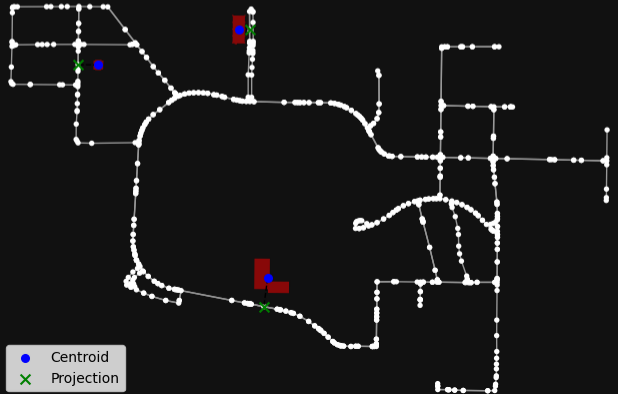
\includegraphics[width=\linewidth]{figures/fig1.png}
        \caption{Graph-based road network.}
        \label{fig:graph}
    \end{subfigure}\hfill
    \begin{subfigure}{0.48\textwidth}
        \centering
        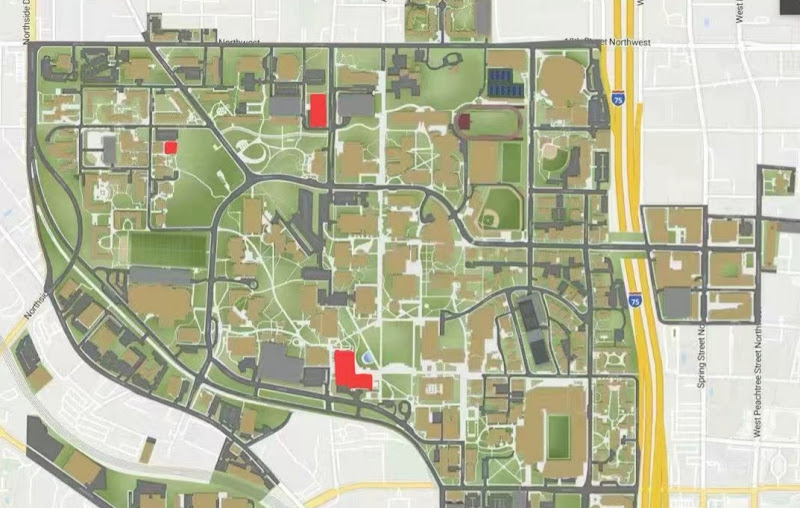
\includegraphics[width=\linewidth]{figures/fig2.jpg}
        \caption{Campus map with buildings.}
        \label{fig:map}
    \end{subfigure}
    \caption{Comparison between the road network representation and the campus map.}
    \label{fig:campus-comparison}
\end{figure}

\section*{Algorithms}
% This part is drafted by Fred Yang.
\subsection*{Graph Representation}
The Georgia Tech Navigation System is modeled as a weighted, directed graph $G = (V, E)$, where
\begin{itemize}
    \item $V$ denotes the vertex (node) set representing the road intersections, curve points along road segments, and projected building point on the road.
    \item $E$ denotes the edge set representing the road segments weighted by haversine distance. For two-way streets, edges are inserted in both directions while for one-way streets only a single directed edge is created.
\end{itemize}
Given that the Georgia Tech road network is a sparse graph with most intersections connecting to only a handful of roads, instead of storing the graph as a adjacency matrix which requires $O(|V|^2)$ for storage, adjacency list (which requires $O(|V|+|E|)$ for storage) is a more natural and efficient choice in this case. Besides, it is also easy to establish an adjacency list since the extracted nodes from OSM have a \texttt{neighbors} tag.

\subsection*{A* Search}

Unlike exhaustive methods such as Breadth-First Search or Dijkstra’s Algorithm, which may expand nearly all nodes in the graph, A* improves efficiency with heuristic-guided approach.

A* search algorithm evaluates nodes by using the function:
\[
f(n) = g(n)+h(n),
\]
where $g(n)$ represents the exact cost of the path from the starting point to any vertex $n$, and $h(n)$ represents the heuristic estimated cost from vertex $n$ to the goal. Each time through the main loop, it examines the vertex $n$ with lowest $f(n)$.

In this case, we use the haversine distance from a vertex to the destination as the heuristic
\[
h(n) =  2R \cdot \arcsin\!\left( \sqrt{ \sin^2\!\left(\frac{\phi_2 - \phi_1}{2}\right) + \cos(\phi_1)\cos(\phi_2)\sin^2\!\left(\frac{\lambda_2 - \lambda_1}{2}\right) } \right),
\] where $R$ denotes the radius of the Earth, $\phi$ denotes the latitude and $\lambda$ denotes the longitude.

\subsection*{Route Metrics}
For each query, the algorithm outputs:
\begin{itemize}
    \item \textbf{Shortest-path distance} (i.e. sum of edge weights).
    \item \textbf{Estimated travel time} $t = d/v$, where $v$ is assumed average vehicle speed.
    \item \textbf{Node sequence}: ordered list of graph vertices along the path.
    \item \textbf{Edge sequence}: road segments traversed with distances.
\end{itemize}

\subsection*{Turn-by-Turn Instruction Generation}

To convert raw node sequences into human-readable directions, we utilize the bearing angles $\theta$ between consecutive edges, and determine the instruction by a function $\text{intersection}(\theta)$:
\[
\text{Instruction}(\theta) =
\begin{cases}
\text{Straight}, & |\theta| < 30^\circ \\[6pt]
\text{Left Turn}, & 30^\circ \leq \theta < 150^\circ \ \wedge \ \text{cross}(\mathbf{e}_1,\mathbf{e}_2) > 0 \\[6pt]
\text{Right Turn}, & 30^\circ \leq \theta < 150^\circ \ \wedge \ \text{cross}(\mathbf{e}_1,\mathbf{e}_2) < 0 \\[6pt]
\text{U-turn}, & |\theta| \geq 150^\circ
\end{cases}
\]
where $\mathbf{e}_1, \mathbf{e}_2$ are consecutive edge vectors, $\theta = \arccos\!\left( \dfrac{\mathbf{e}_1 \cdot \mathbf{e}_2}{\|\mathbf{e}_1\|\|\mathbf{e}_2\|} \right)$, and $\text{cross}(\mathbf{e}_1,\mathbf{e}_2)$ is the determinant of 2 by 2 matrix formed by two edge vector. 

These thresholds reflect human perception, reducing false turn instructions from slight bends while still capturing sharp changes in direction.

\section*{Platform(s) / modalities of development}

The navigation system will be primarily implemented in \textbf{C} (conforming to the C17 standard), with compilation and testing by \textbf{Clang (macOS)} for development and testing. \textbf{Python 3.10+} is also used for preprocessing and visualizing (if needed) OSM data. Development is managed collaboratively through \textbf{GitHub} and \textbf{Overleaf}, ensuring consistent version control of both source code and \LaTeX{} documentation throughout project.

% Last Page
\newpage
\section*{Acknowledgment}
We appreciate each teammate hard work and positive cooperation for the checkpoint1:
\begin{itemize}
    \item Jing He and Haowen Jiang: handled the campus data processing, graph modeling, and wrote Data Description
    \item Ming Fan and Chia-Hsin Chiu: set up Github, co-authered the abstract, introduction, literature review, objectives and system descriptions part.
    \item Fred Yang: proposed and wrote the algorithmic part, converted the draft report from Google Docx to \LaTeX{}, and helped set up the GitHub/Overleaf repository for future team collaboration.
\end{itemize}
We thank the Georgia Tech CSE 6010 teaching staff for their guidance during the early stages of this project.  
The current implementation and progress can be found at:  
\url{https://github.com/fredkyang/gt_cse6010_navigation_system}

This repository is intended solely for use in CSE 6010 (Fall 25) coursework.

About AI: literature review is summarized by AI.
\bibliographystyle{unsrt}
\bibliography{references}

\end{document}